\chapter{Simulations}
This chapter presents the results obtained by simulations. The research has been made for two models
described in chapter \ref{ch:model}. The motion planning problem has been solved using endogenous
configuration space approach presented in chapter \ref{ch:endogen}.

There are some issues that are common regardless the studied object. Moreover,
both RobRex mobile manipulator and unicycle have two control inputs. That is why
the same control functions representation may be used in those two models.
The base used to represent the control functions was trigonometric, including up to the third harmonics, that means
\begin{equation}
\Psi=\begin{pmatrix}
1 & \sin(\omega t) & \cos(\omega t)& \sin(2\omega t) & \cos(2\omega t)& \sin(3\omega t) & \cos(3\omega t)
\end{pmatrix},
\end{equation}
where $\omega=\frac{2\pi}{T}$ and $T$ is the control horizon. Assuming the above and the fact that the model is controlled by two inputs, the matrix $P(t)$ in \eqref{eq:Pt} is of the form
\begin{equation}
P(t)=\begin{bmatrix}
\Psi & 0_{1\times 7}\\
0_{1\times 7} & \Psi
\end{bmatrix}.
\end{equation}
The decay rate $\gamma$ in \eqref{eq:endogen_num} has been set to $0.05$ for all
the simulations demonstrated in this chapter.


\section{Unicycle}
The model of the unicycle has been implemented in order to examine the behaviour
of the motion planning algorithm for a very simple object with discontinuities. 

\subsection{Problem formulation}
The motion planning problem to be solved is kind of a parking manoeuvre. The initial
state of the manipulator is $q_0 = [w_0; \dot{w_0}] = (0, 0, R\frac{\pi}{2}, 0_5)^T$
and the desired end state is $q_d = [w_d; \dot{w_d}] = (10, 0, a\frac{\pi}{2}, 0_5)^T$.
The motion is supposed to be executed within the fixed control horizon $T$.

\subsection{Simulation conditions}
The parameters of the object used during the simulation are:
\begin{multicols}{2}
\begin{itemize}
\item $m= \,\mathrm{kg}$,
\item $R= \,\mathrm{m}$,
\item $I_\phi =\,\mathrm{kgm^2}$,
\item $I_\theta =\,\mathrm{kgm_2}$.
\end{itemize}
\end{multicols}


\section{Mobile platform}
\subsection{Problem formulation}
\label{sec:rex_task}
The problem to be solved is to move the platform from the initial state
$q_0 = [w_0; \dot{w}_0] = (0, 0, a\frac{\pi}{2}, 0_7)^T$ to the desired state
$q_d = [w_d; \dot{w}_d] = (10, 0, a\frac{\pi}{2}, 0_7)^T$
within the given amount of time $T$. 
This corresponds to a parking manoeuvre.

Now two types of friction models will be discussed --- linear
and discontinuous. These models will be employed in simulations
regarding solving the above problem.

\subsection{Simulation conditions}
The object parameters were set according to \cite{coupled} and are as follows:
\begin{multicols}{2}
\begin{itemize}
\item $m_p = 21.107\,\mathrm{kg}$,
\item $m_w = 2.380\,\mathrm{kg}$,
\item $a_{p1} = 0.377\,\mathrm{m}$,
\item $a_{p2} = 0.008\,\mathrm{m}$,
\item $a = 0.730\,\mathrm{m}$,
\item $b = 0.350\,\mathrm{m}$,
\item $R = 0.127\,\mathrm{m}$,
\item $I_{p33} = 1.991\,\mathrm{kgm^2}$,
\item $I_{w11} = 0.015\,\mathrm{kgm^2}$,
\item $I_{w33} = 0.009\,\mathrm{kgm^2}$.
\end{itemize}
\end{multicols}
\setcounter{MaxMatrixCols}{14}
Initial conditions for the $\lambda$ parameters used to compute control functions
in \eqref{eq:endogen_num} are
\begin{equation}
\lambda_0=
(\underbrace{0, \ 0.5, \ 0, \ 0, \ 0, \ 0, \ 0,}_{u_1}\ \underbrace{0, \ 0.5, \ 0, \ 0, \ 0, \ 0, \ 0}_{u_2})^T,
\end{equation}
i.e. only first harmonic sines are used.
 	

\subsection{Linear friction model}
This model assumes that coefficients $\epsilon_i$ and $\tau_i$ in \eqref{eq:force_r} are constant. Four cases of friction coefficients values have been analysed:
\begin{enumerate}
\item $\epsilon_i=15$ and $\tau_i=15$,
\item $\epsilon_i=15$ and $\tau_i=1$,
\item $\epsilon_i=1$ and $\tau_i=15$,
\item $\epsilon_i=1$ and $\tau_i=1$,
\end{enumerate}
for $i=1,\,2,\,3,\,4$.
Every case was studied with two different time horizons 10\,s and 20\,s. The results of the simulations are shown in figures ...

It is also worth to check whether the input functions obtained through the algorithm are feasible on the real object. The total energy of the signal was computed as $\int_0^T u^2\ud t$ and the maximal amplitude which can be compared to the maximum torque achievable by the real actuator. These values computed for all the simulations run are presented in table \ref{tab:control}.
\begin{table}[h]
\centering
\caption{My caption}
\label{tab:control} %TODO put proper values
\begin{tabular}{rr|r|r|r|r|}
\cline{3-6}
\multicolumn{1}{c}{}                      & \multicolumn{1}{c|}{}           & \multicolumn{2}{c|}{energy}                             & \multicolumn{2}{c|}{amplitude}                          \\ \hline
\multicolumn{1}{|c|}{$\tau$}              & \multicolumn{1}{c|}{$\epsilon$} & \multicolumn{1}{c|}{$u_1$} & \multicolumn{1}{c|}{$u_2$} & \multicolumn{1}{c|}{$u_1$} & \multicolumn{1}{c|}{$u_2$} \\ \hline
\multicolumn{1}{|r|}{\multirow{2}{*}{15}} & 15                              &                            &                            &                            &                            \\ \cline{2-6} 
\multicolumn{1}{|r|}{}                    & 1                               &                            &                            &                            &                            \\ \hline
\multicolumn{1}{|r|}{\multirow{2}{*}{1}}  & 15                              &                            &                            &                            &                            \\ \cline{2-6} 
\multicolumn{1}{|r|}{}                    & 1                               &                            &                            &                            &                            \\ \hline
\end{tabular}
\end{table}
\begin{figure}[h]
\begin{subfigure}[b]{\textwidth}
\centering
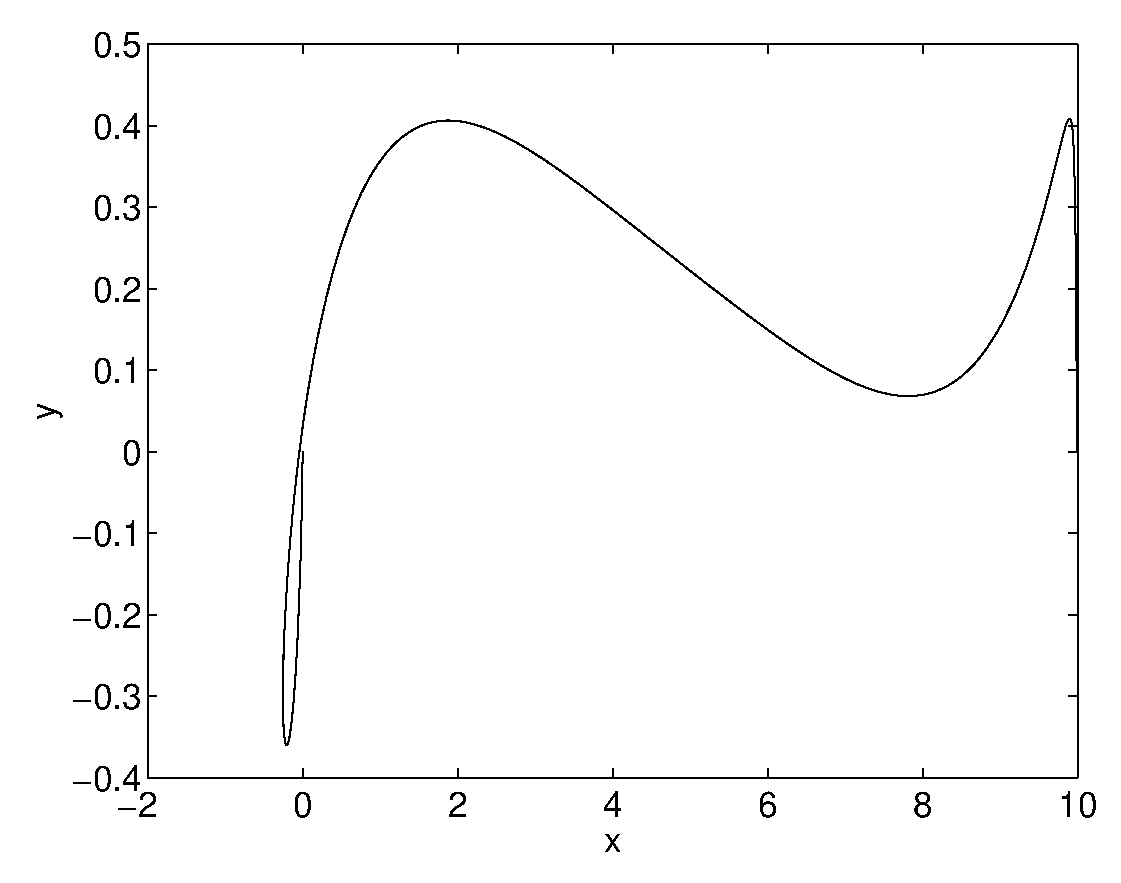
\includegraphics[height=0.3\textheight]{img/final_15_1_10_path.eps}
\caption{path}
\end{subfigure}

\begin{subfigure}[b]{\textwidth}
\centering
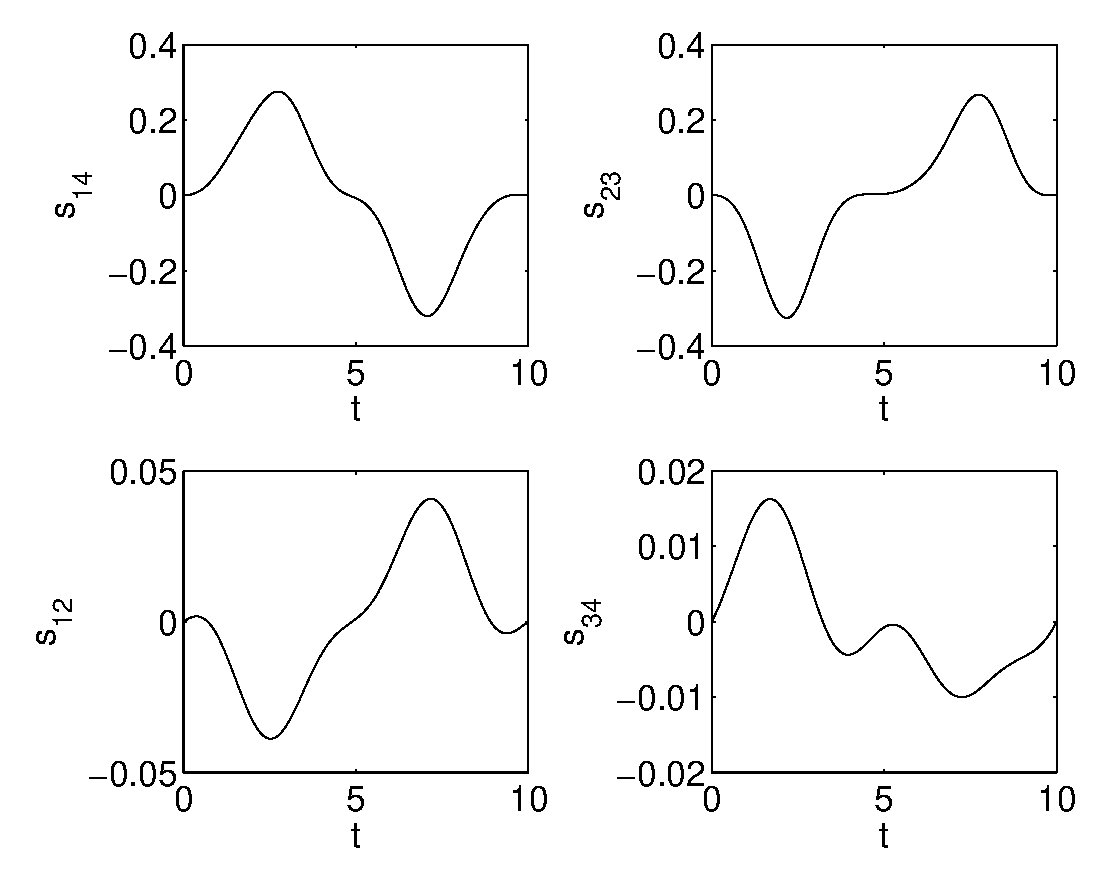
\includegraphics[height=0.3\textheight]{img/final_15_1_10_slips.eps}
\caption{slips}
\end{subfigure}

\begin{subfigure}[b]{\textwidth}
\centering
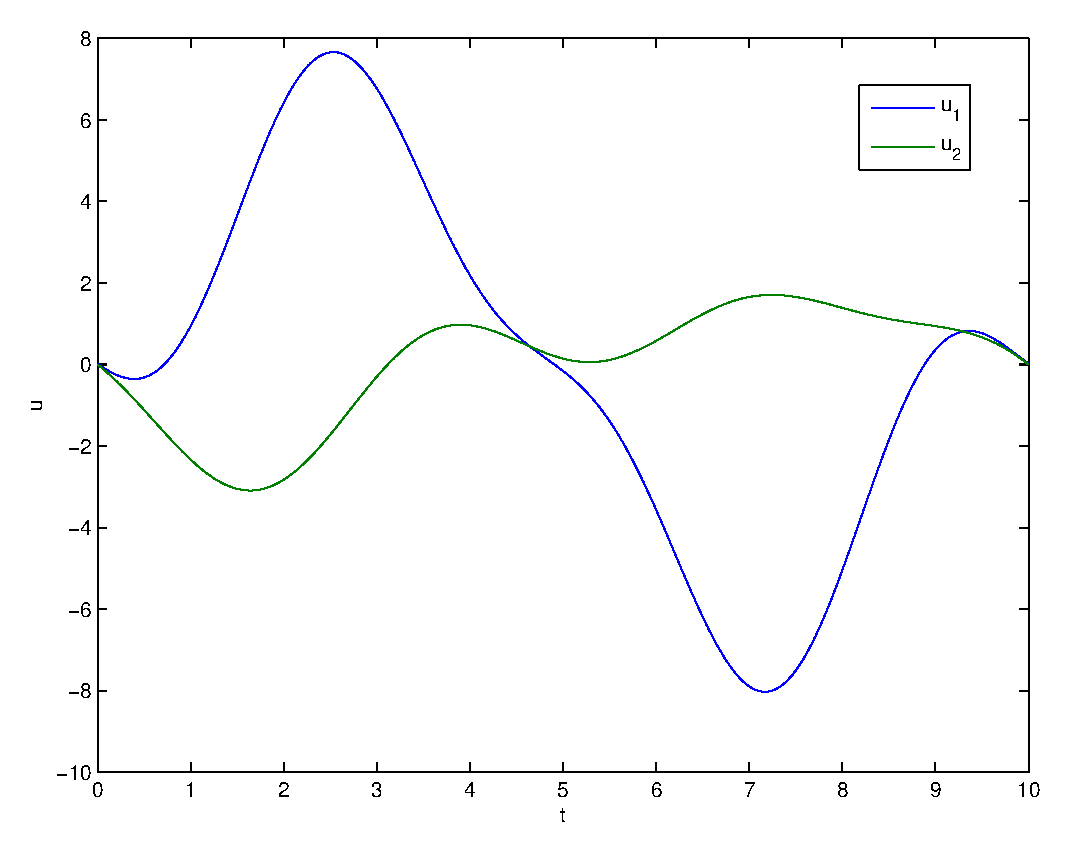
\includegraphics[height=0.3\textheight]{img/final_15_1_10_u.eps}
\caption{path}
\end{subfigure}
\caption{Mobile platform, $\epsilon=15$, $\tau=1$, $T=10$}
\label{fig:pl1}
\end{figure}

\begin{figure}[h]
\begin{subfigure}[b]{\textwidth}
\centering
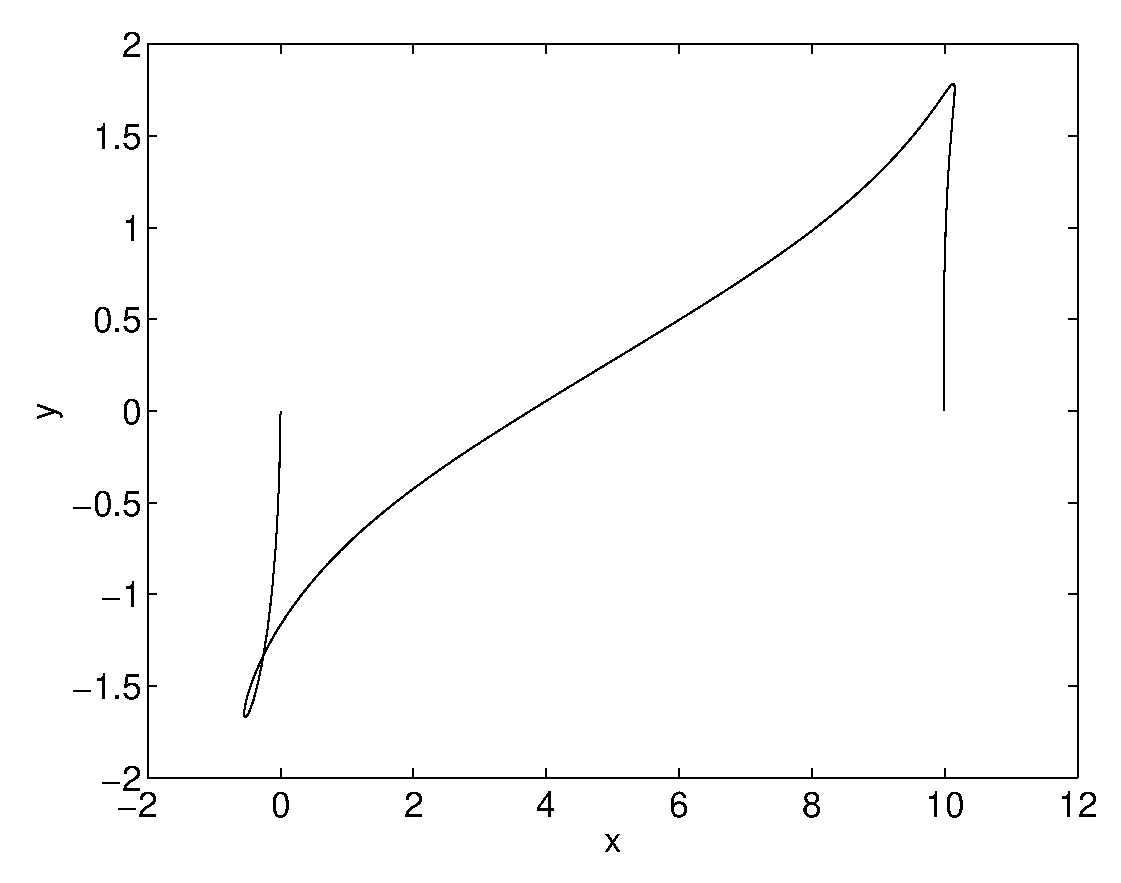
\includegraphics[height=0.3\textheight]{img/final_15_1_20_path.eps}
\caption{path}
\end{subfigure}

\begin{subfigure}[b]{\textwidth}
\centering
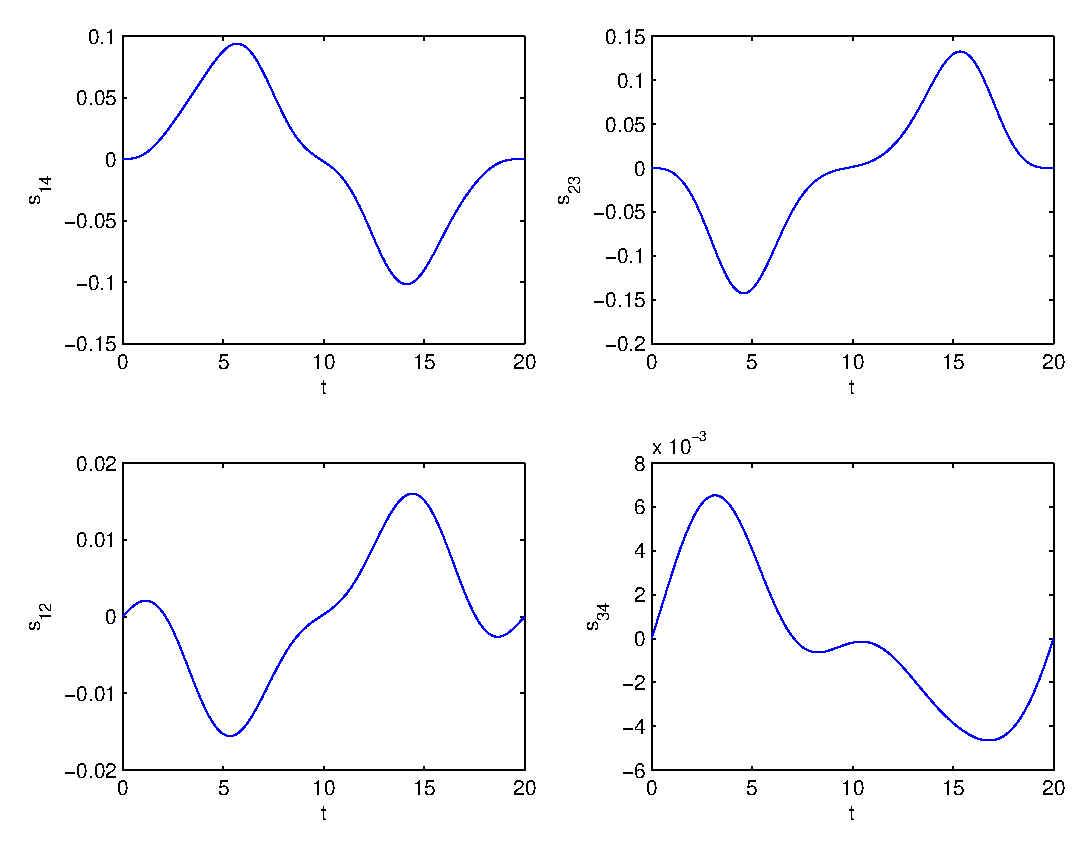
\includegraphics[height=0.3\textheight]{img/final_15_1_20_slips.eps}
\caption{slips}
\end{subfigure}

\begin{subfigure}[b]{\textwidth}
\centering
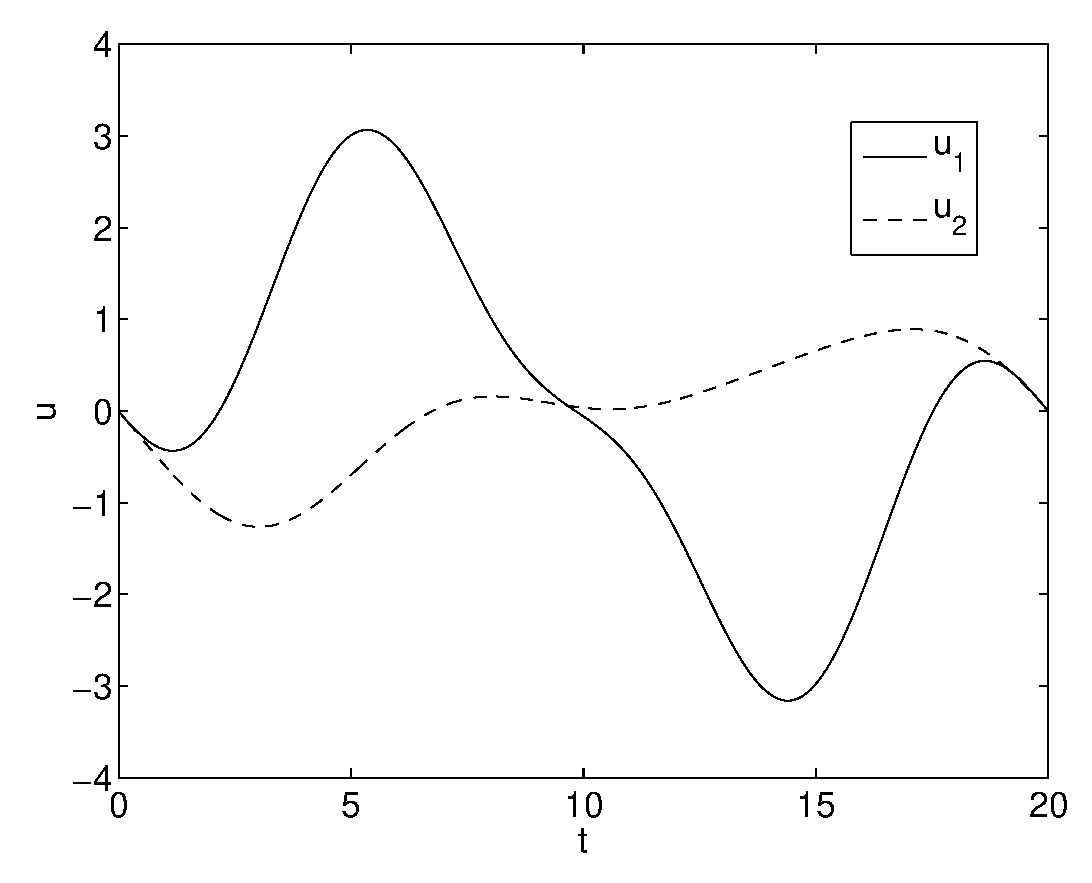
\includegraphics[height=0.3\textheight]{img/final_15_1_20_u.eps}
\caption{path}
\end{subfigure}
\caption{Mobile platform, $\epsilon=15$, $\tau=1$, $T=20$}
\label{fig:pl2}
\end{figure}

%%%%%%%%%%%%%%%%%%%%%%%%%%%%%%%%%%%%%%%%%%%%%%%%%%%%%%%%%%%%%%%%%%%%%%%%%%%%%%%%%%%%%%%%%%%
%%%%%%%%%%%%%%%%%%%%%%%%%%%%%%%%%%%%%%%%%%%%%%%%%%%%%%%%%%%%%%%%%%%%%%%%%%%%%%%%%%%%%%%%%%%
%%%%%%%%%%%%%%%%%%%%%%%%%%%%%%%%%%%%%%%%%%%%%%%%%%%%%%%%%%%%%%%%%%%%%%%%%%%%%%%%%%%%%%%%%%%
%%%%%%%%%%%%%%%%%%%%%%%%%%%%%%%%%%%%%%%%%%%%%%%%%%%%%%%%%%%%%%%%%%%%%%%%%%%%%%%%%%%%%%%%%%%
%%%%%%%%%%%%%%%%%%%%%%%%%%%%%%%%%%%%%%%%%%%%%%%%%%%%%%%%%%%%%%%%%%%%%%%%%%%%%%%%%%%%%%%%%%%

\begin{figure}[h]
\begin{subfigure}[b]{\textwidth}
\centering
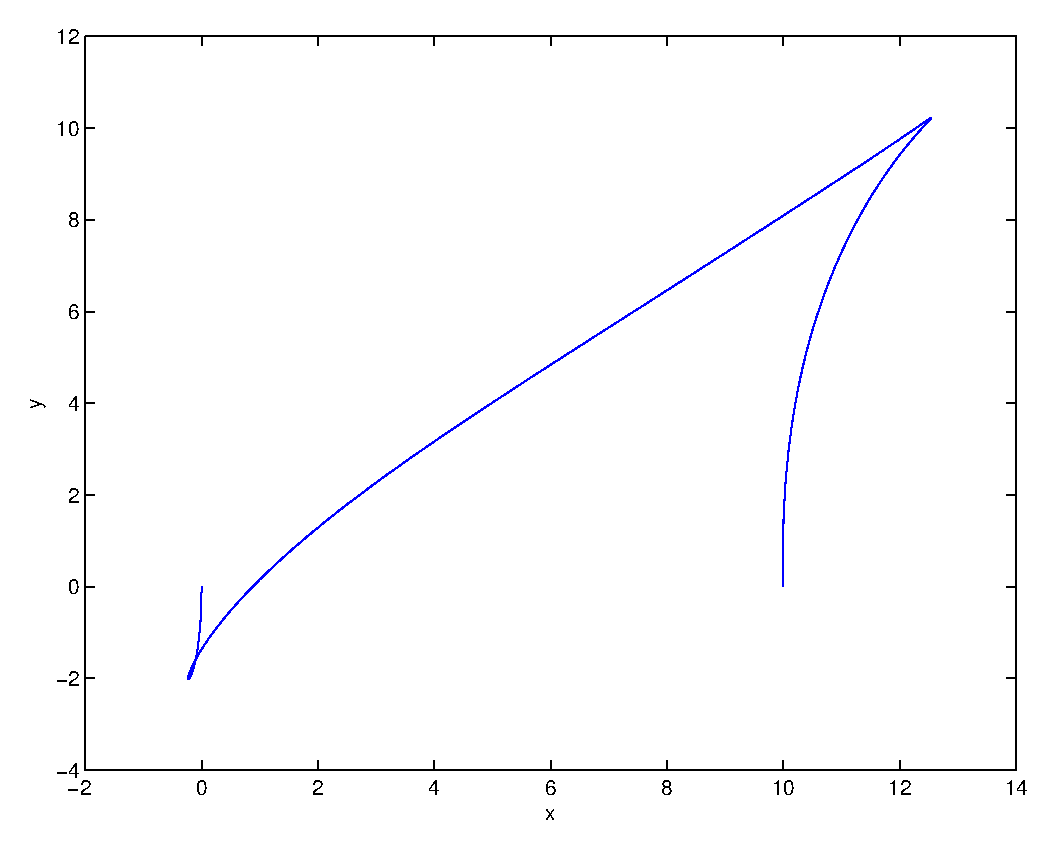
\includegraphics[height=0.3\textheight]{img/final_15_15_10_path.eps}
\caption{path}
\end{subfigure}

\begin{subfigure}[b]{\textwidth}
\centering
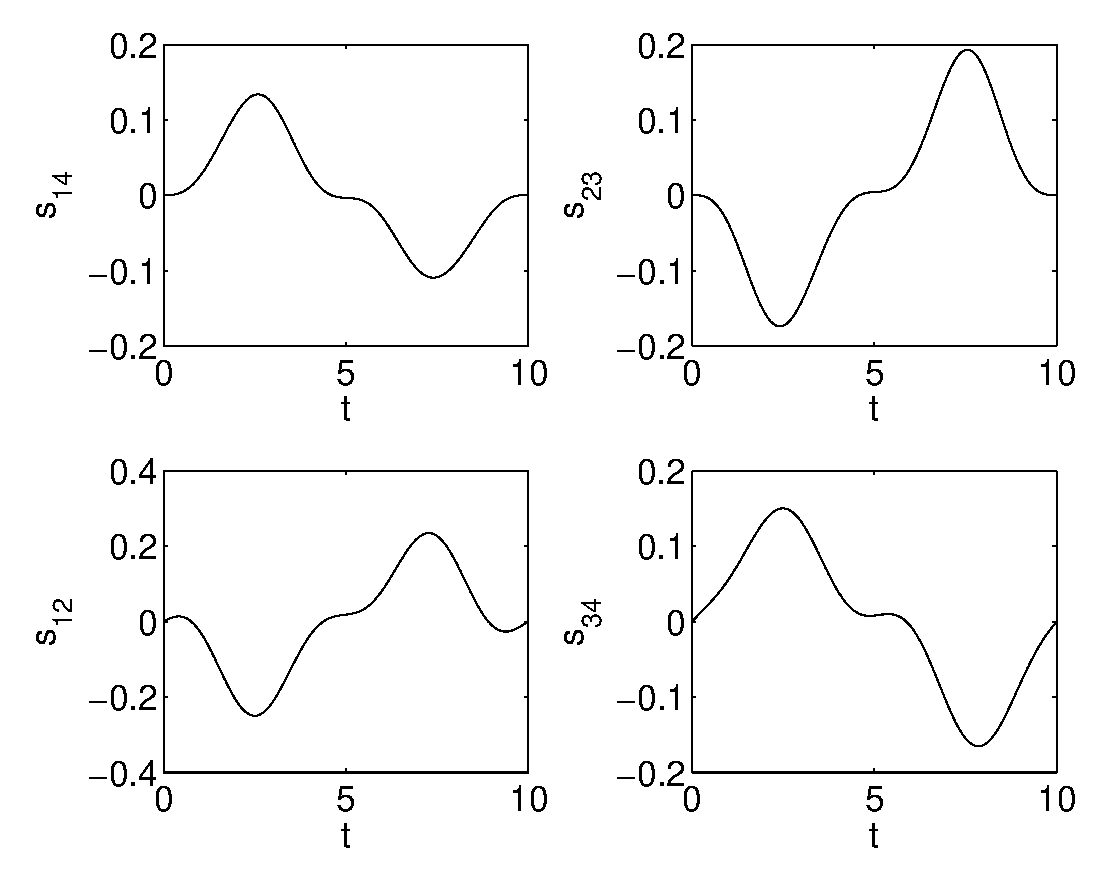
\includegraphics[height=0.3\textheight]{img/final_15_15_10_slips.eps}
\caption{slips}
\end{subfigure}

\begin{subfigure}[b]{\textwidth}
\centering
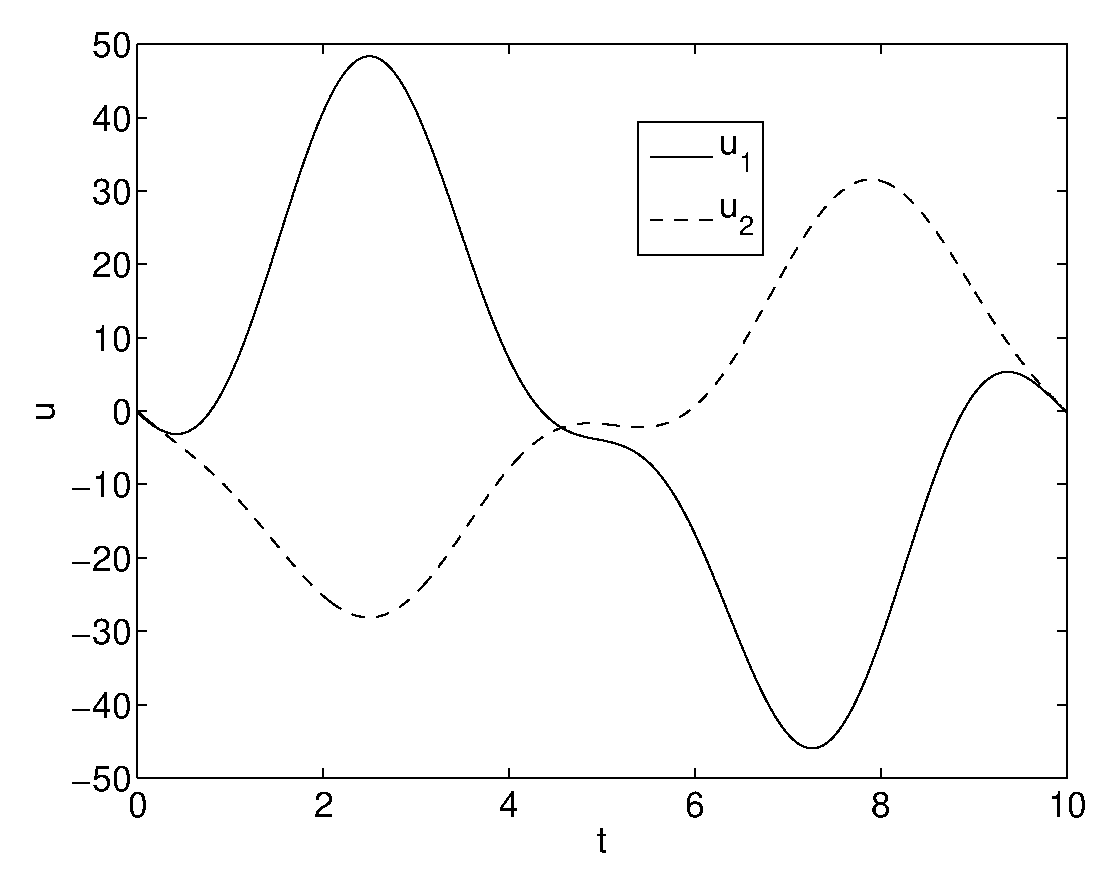
\includegraphics[height=0.3\textheight]{img/final_15_15_10_u.eps}
\caption{path}
\end{subfigure}
\caption{Mobile platform, $\epsilon=15$, $\tau=15$, $T=10$}
\label{fig:pl3}
\end{figure}

\begin{figure}[h]
\begin{subfigure}[b]{\textwidth}
\centering
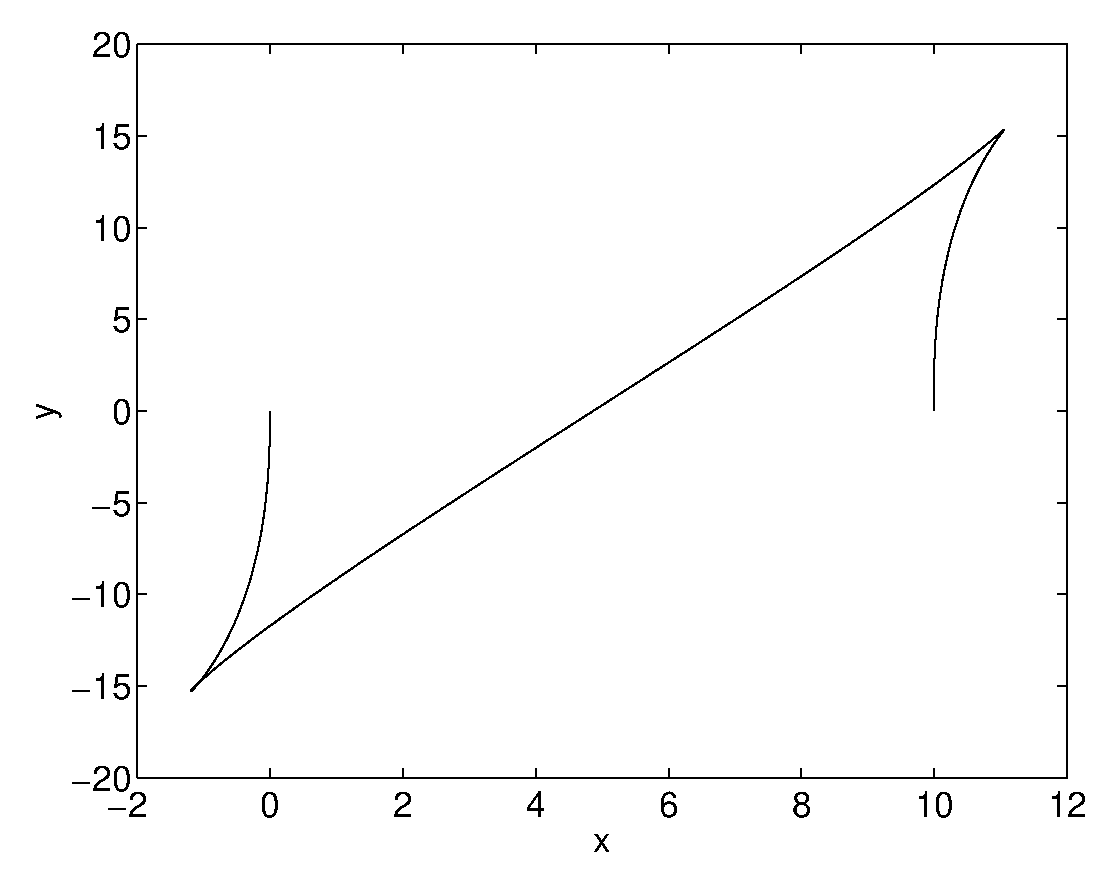
\includegraphics[height=0.3\textheight]{img/final_15_15_20_path.eps}
\caption{path}
\end{subfigure}

\begin{subfigure}[b]{\textwidth}
\centering
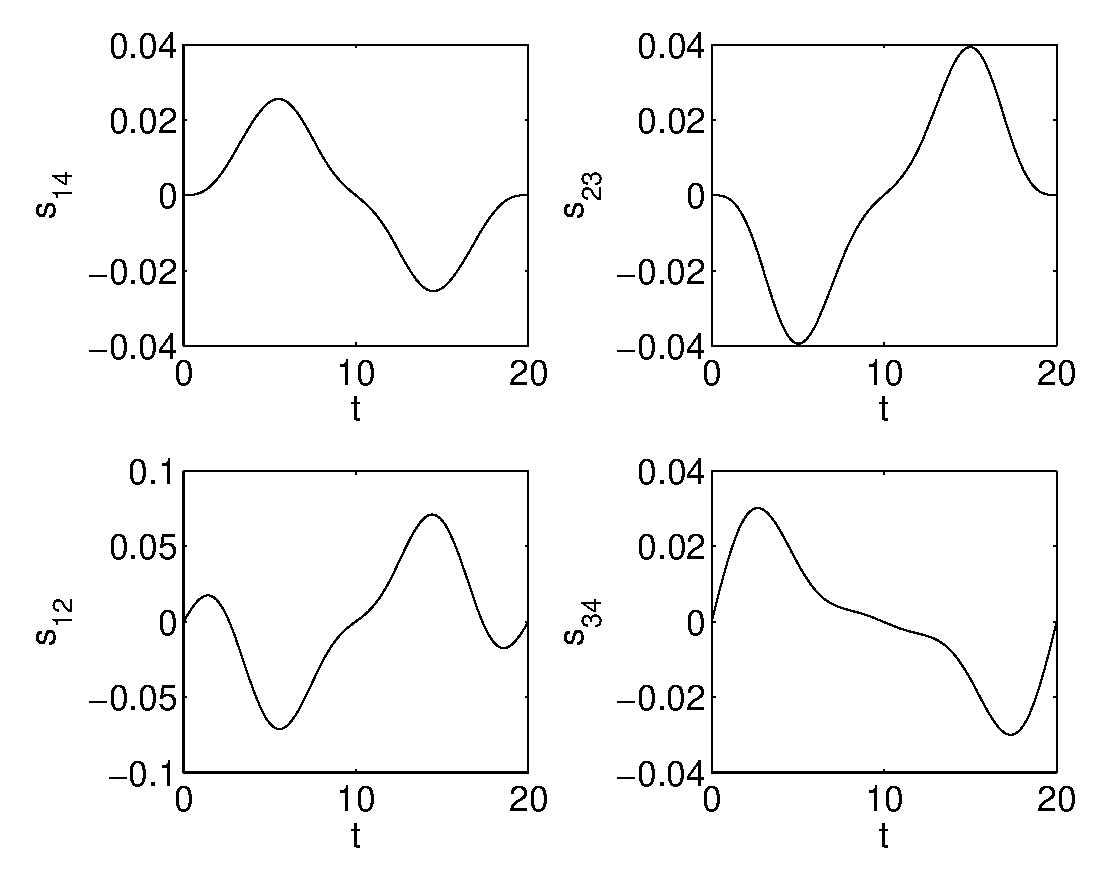
\includegraphics[height=0.3\textheight]{img/final_15_15_20_slips.eps}
\caption{slips}
\end{subfigure}

\begin{subfigure}[b]{\textwidth}
\centering
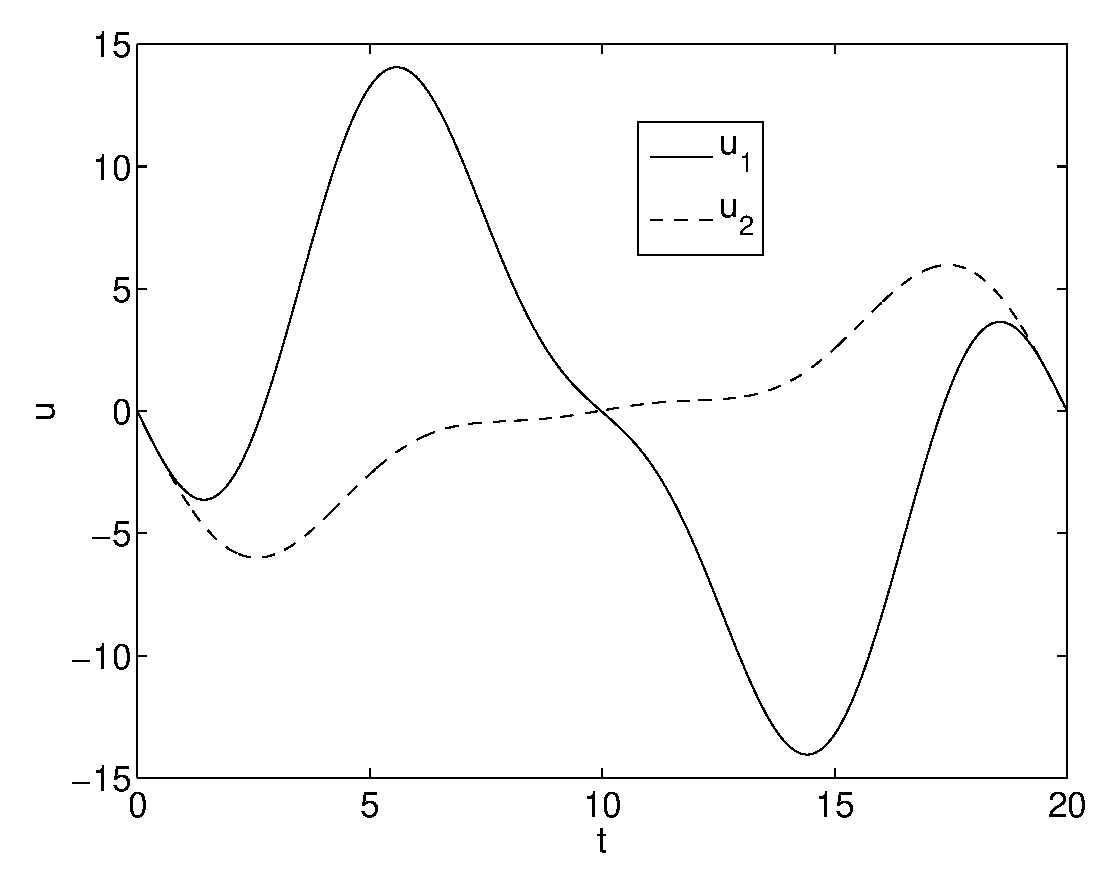
\includegraphics[height=0.3\textheight]{img/final_15_15_20_u.eps}
\caption{path}
\end{subfigure}
\caption{Mobile platform, $\epsilon=15$, $\tau=15$, $T=20$}
\label{fig:pl4}
\end{figure}

%%%%%%%%%%%%%%%%%%%%%%%%%%%%%%%%%%%%%%%%%%%%%%%%%%%%%%%%%%%%%%%%%%%%%%%%%%%%%%%%%%%%%%%%%%%
%%%%%%%%%%%%%%%%%%%%%%%%%%%%%%%%%%%%%%%%%%%%%%%%%%%%%%%%%%%%%%%%%%%%%%%%%%%%%%%%%%%%%%%%%%%
%%%%%%%%%%%%%%%%%%%%%%%%%%%%%%%%%%%%%%%%%%%%%%%%%%%%%%%%%%%%%%%%%%%%%%%%%%%%%%%%%%%%%%%%%%%
%%%%%%%%%%%%%%%%%%%%%%%%%%%%%%%%%%%%%%%%%%%%%%%%%%%%%%%%%%%%%%%%%%%%%%%%%%%%%%%%%%%%%%%%%%%
%%%%%%%%%%%%%%%%%%%%%%%%%%%%%%%%%%%%%%%%%%%%%%%%%%%%%%%%%%%%%%%%%%%%%%%%%%%%%%%%%%%%%%%%%%%
\begin{figure}[h]
\begin{subfigure}[b]{\textwidth}
\centering
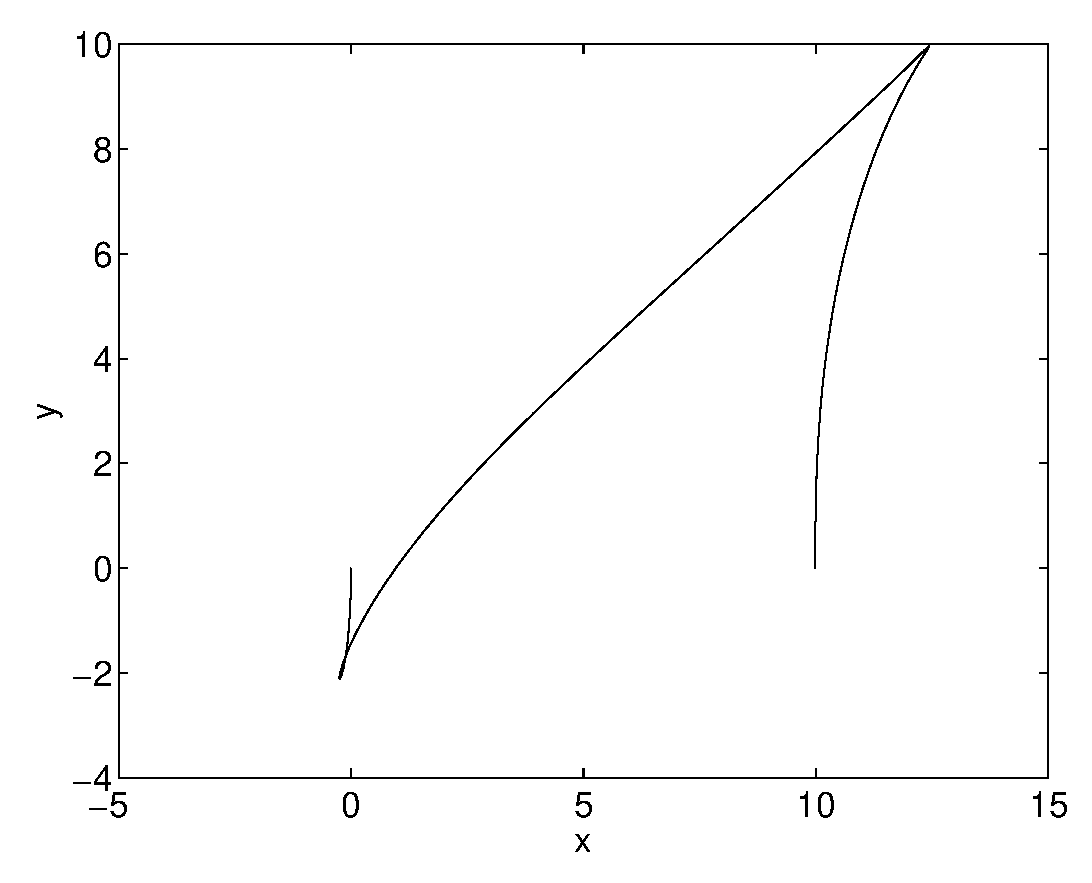
\includegraphics[height=0.3\textheight]{img/final_1_15_10_path.eps}
\caption{path}
\end{subfigure}

\begin{subfigure}[b]{\textwidth}
\centering
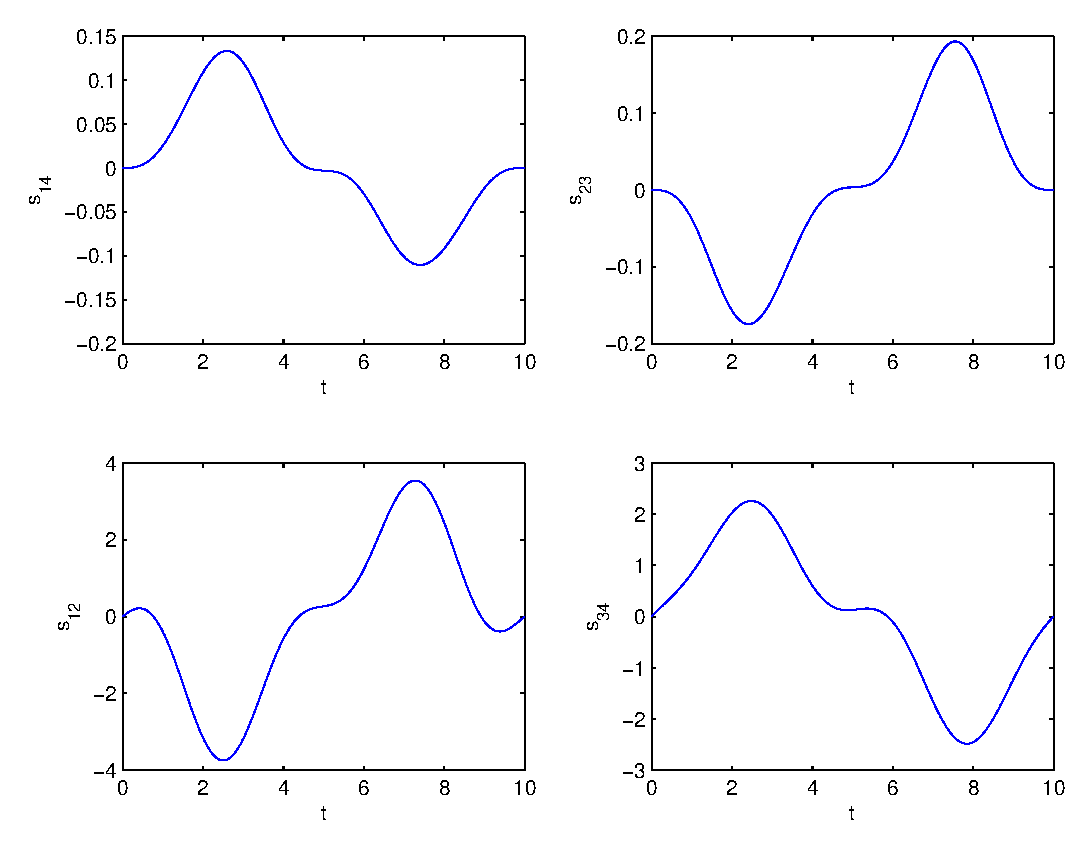
\includegraphics[height=0.3\textheight]{img/final_1_15_10_slips.eps}
\caption{slips}
\end{subfigure}

\begin{subfigure}[b]{\textwidth}
\centering
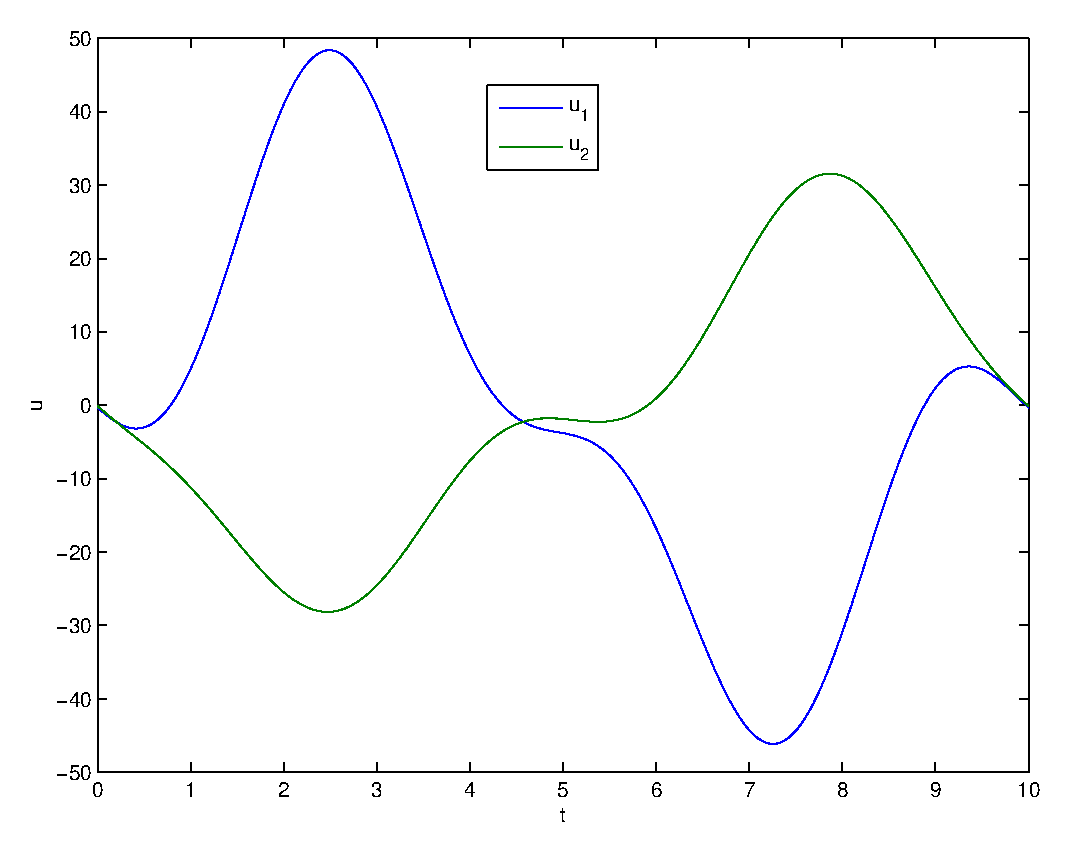
\includegraphics[height=0.3\textheight]{img/final_1_15_10_u.eps}
\caption{path}
\end{subfigure}
\caption{Mobile platform, $\epsilon=1$, $\tau=15$, $T=10$}
\label{fig:pl5}
\end{figure}

\begin{figure}[h]
\begin{subfigure}[b]{\textwidth}
\centering
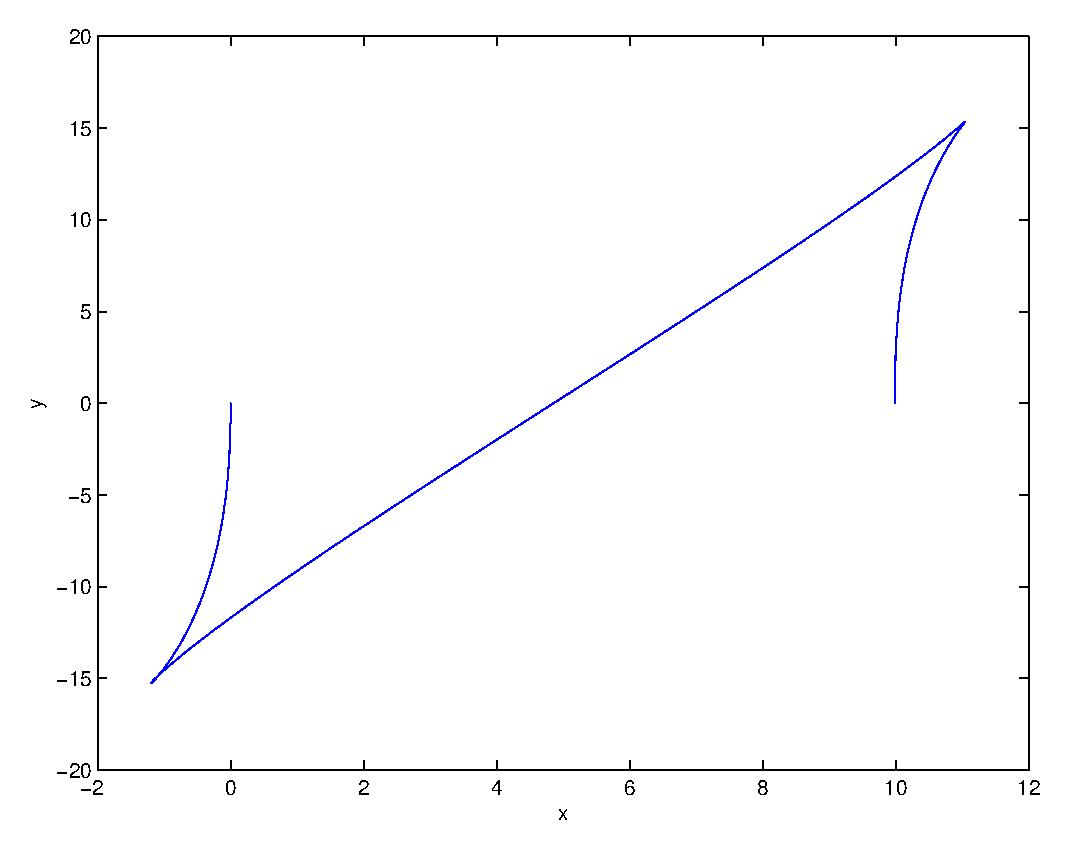
\includegraphics[height=0.3\textheight]{img/final_1_15_20_path.eps}
\caption{path}
\end{subfigure}

\begin{subfigure}[b]{\textwidth}
\centering
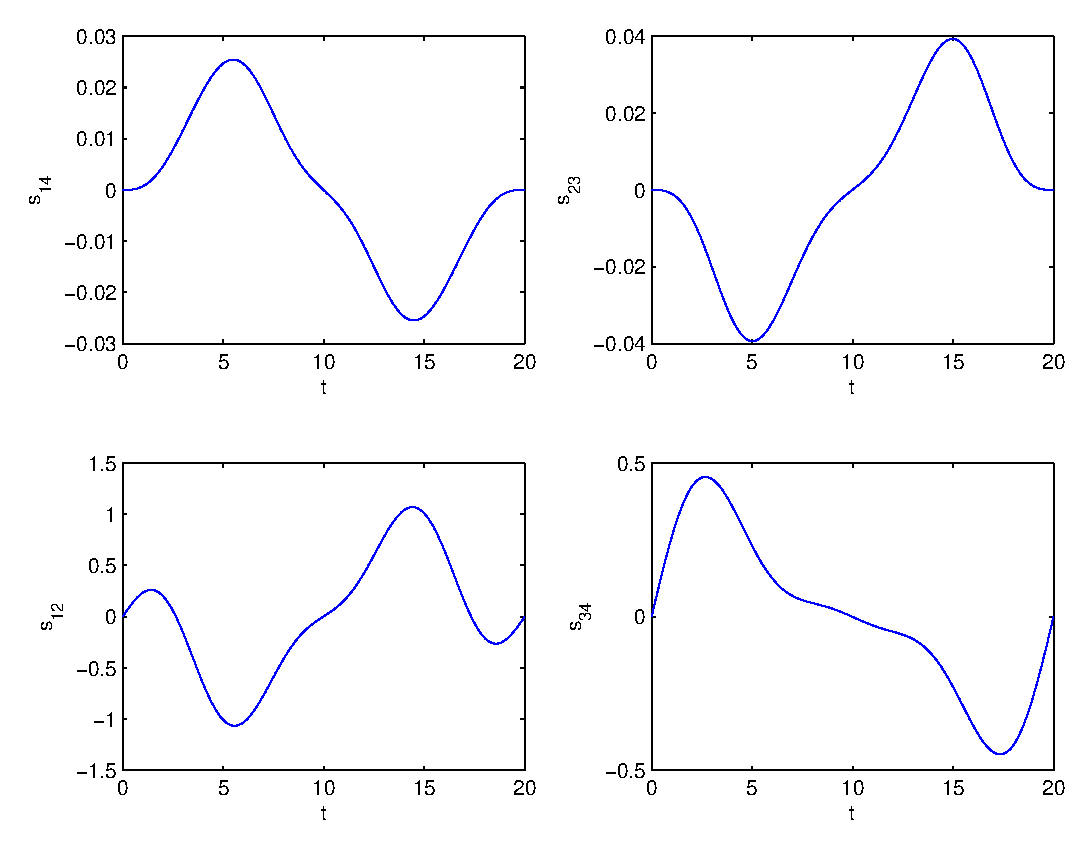
\includegraphics[height=0.3\textheight]{img/final_1_15_20_slips.eps}
\caption{slips}
\end{subfigure}

\begin{subfigure}[b]{\textwidth}
\centering
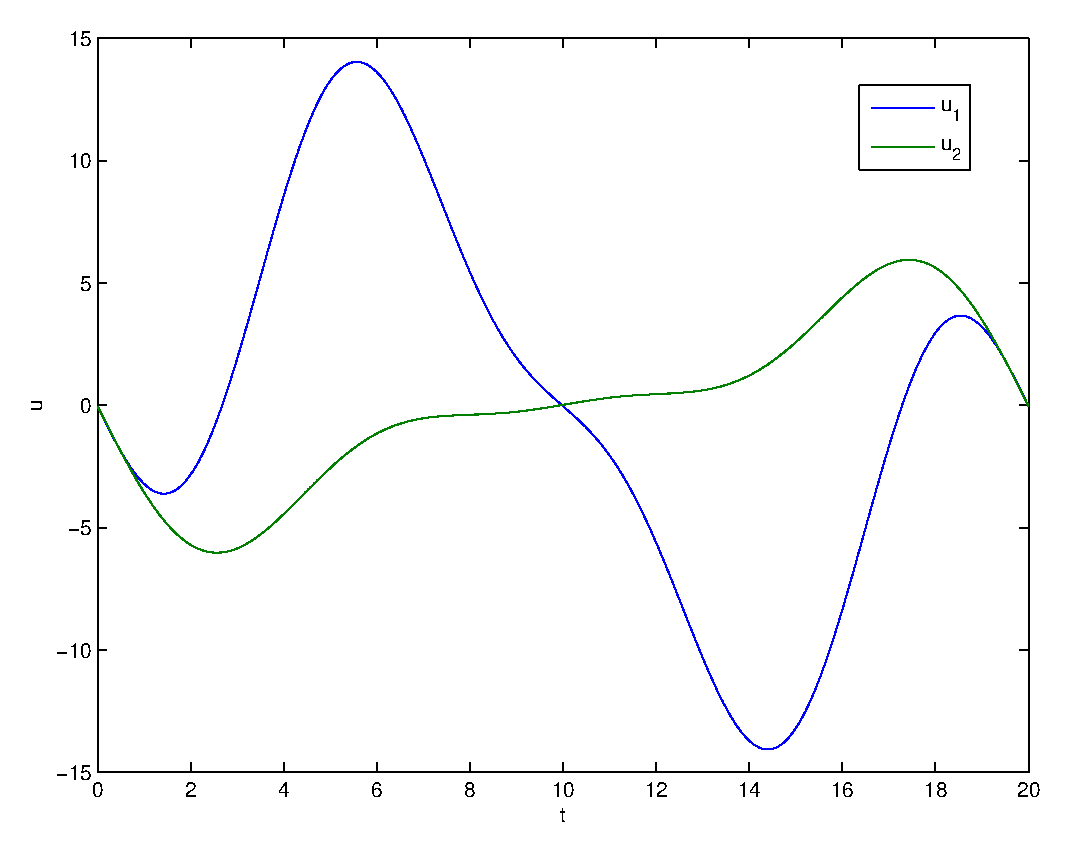
\includegraphics[height=0.3\textheight]{img/final_1_15_20_u.eps}
\caption{path}
\end{subfigure}
\caption{Mobile platform, $\epsilon=1$, $\tau=15$, $T=20$}
\label{fig:pl6}
\end{figure}

%%%%%%%%%%%%%%%%%%%%%%%%%%%%%%%%%%%%%%%%%%%%%%%%%%%%%%%%%%%%%%%%%%%%%%%%%%%%%%%%%%%%%%%%%%%
%%%%%%%%%%%%%%%%%%%%%%%%%%%%%%%%%%%%%%%%%%%%%%%%%%%%%%%%%%%%%%%%%%%%%%%%%%%%%%%%%%%%%%%%%%%
%%%%%%%%%%%%%%%%%%%%%%%%%%%%%%%%%%%%%%%%%%%%%%%%%%%%%%%%%%%%%%%%%%%%%%%%%%%%%%%%%%%%%%%%%%%
%%%%%%%%%%%%%%%%%%%%%%%%%%%%%%%%%%%%%%%%%%%%%%%%%%%%%%%%%%%%%%%%%%%%%%%%%%%%%%%%%%%%%%%%%%%
%%%%%%%%%%%%%%%%%%%%%%%%%%%%%%%%%%%%%%%%%%%%%%%%%%%%%%%%%%%%%%%%%%%%%%%%%%%%%%%%%%%%%%%%%%%
\begin{figure}[h]
\begin{subfigure}[b]{\textwidth}
\centering
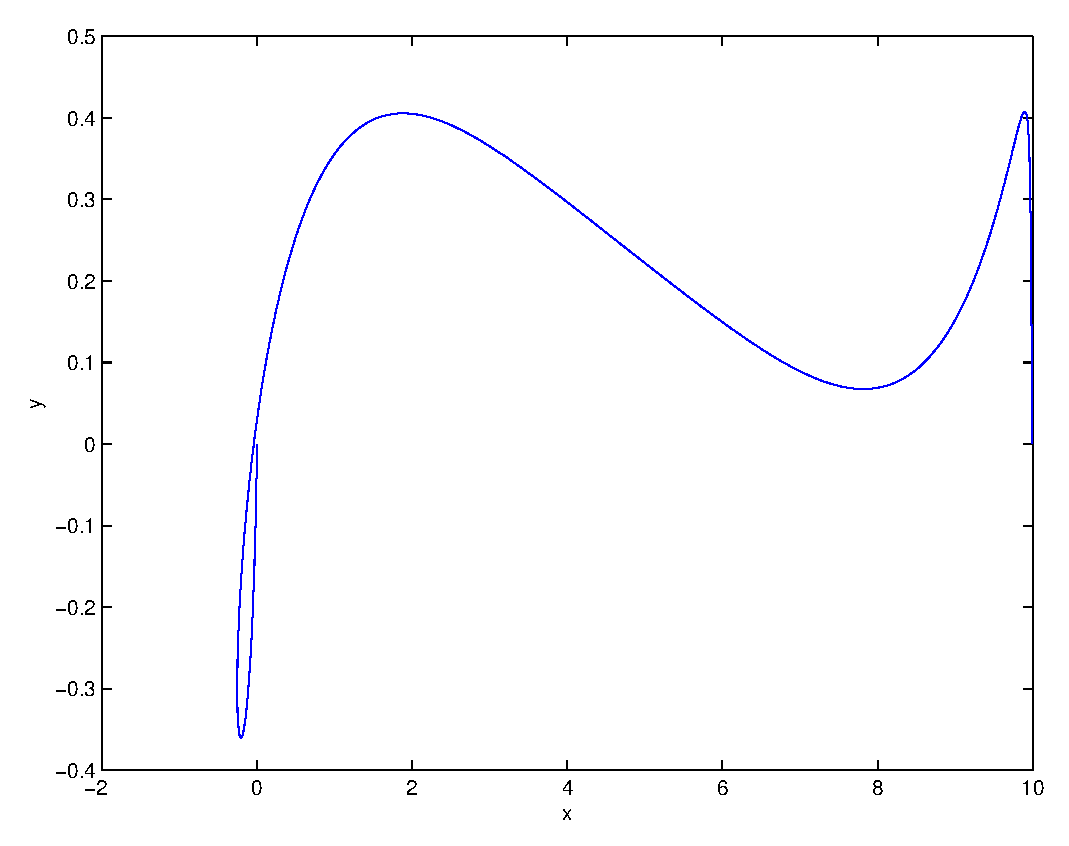
\includegraphics[height=0.3\textheight]{img/final_1_1_10_path.eps}
\caption{path}
\end{subfigure}

\begin{subfigure}[b]{\textwidth}
\centering
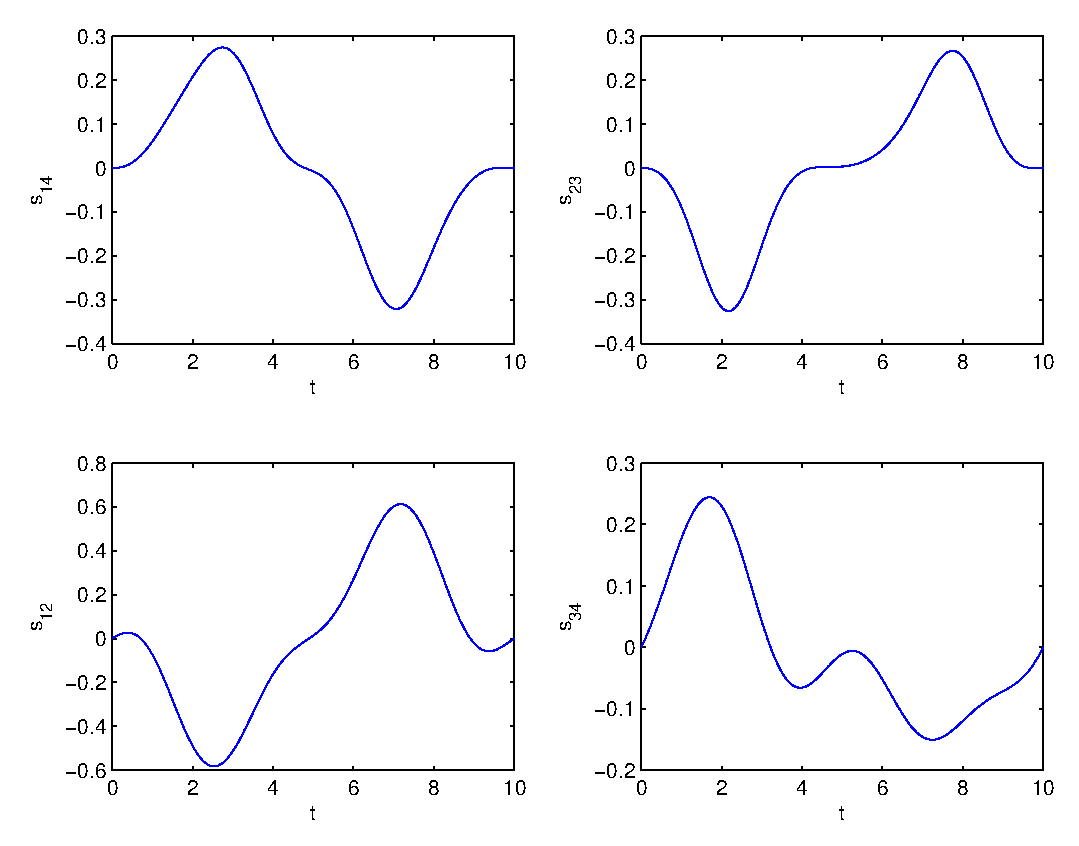
\includegraphics[height=0.3\textheight]{img/final_1_1_10_slips.eps}
\caption{slips}
\end{subfigure}

\begin{subfigure}[b]{\textwidth}
\centering
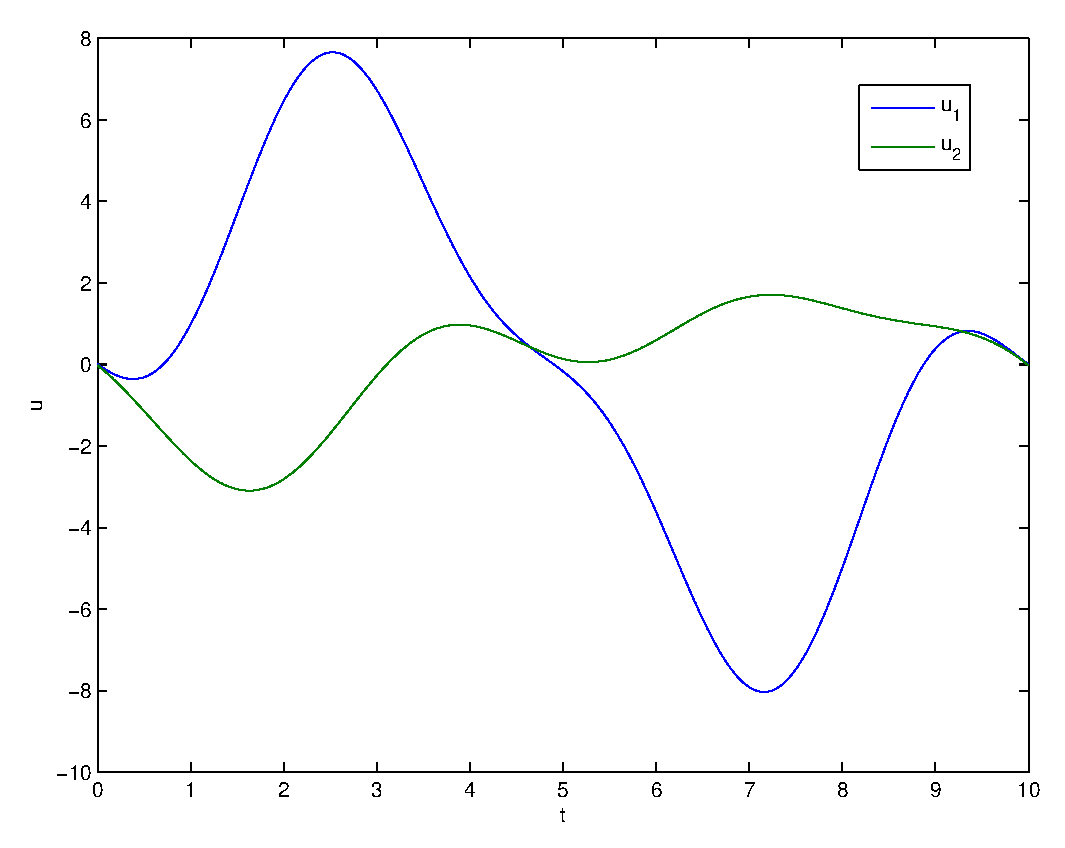
\includegraphics[height=0.3\textheight]{img/final_1_1_10_u.eps}
\caption{path}
\end{subfigure}
\caption{Mobile platform, $\epsilon=1$, $\tau=1$, $T=10$}
\label{fig:pl7}
\end{figure}

\begin{figure}[h]
\begin{subfigure}[b]{\textwidth}
\centering
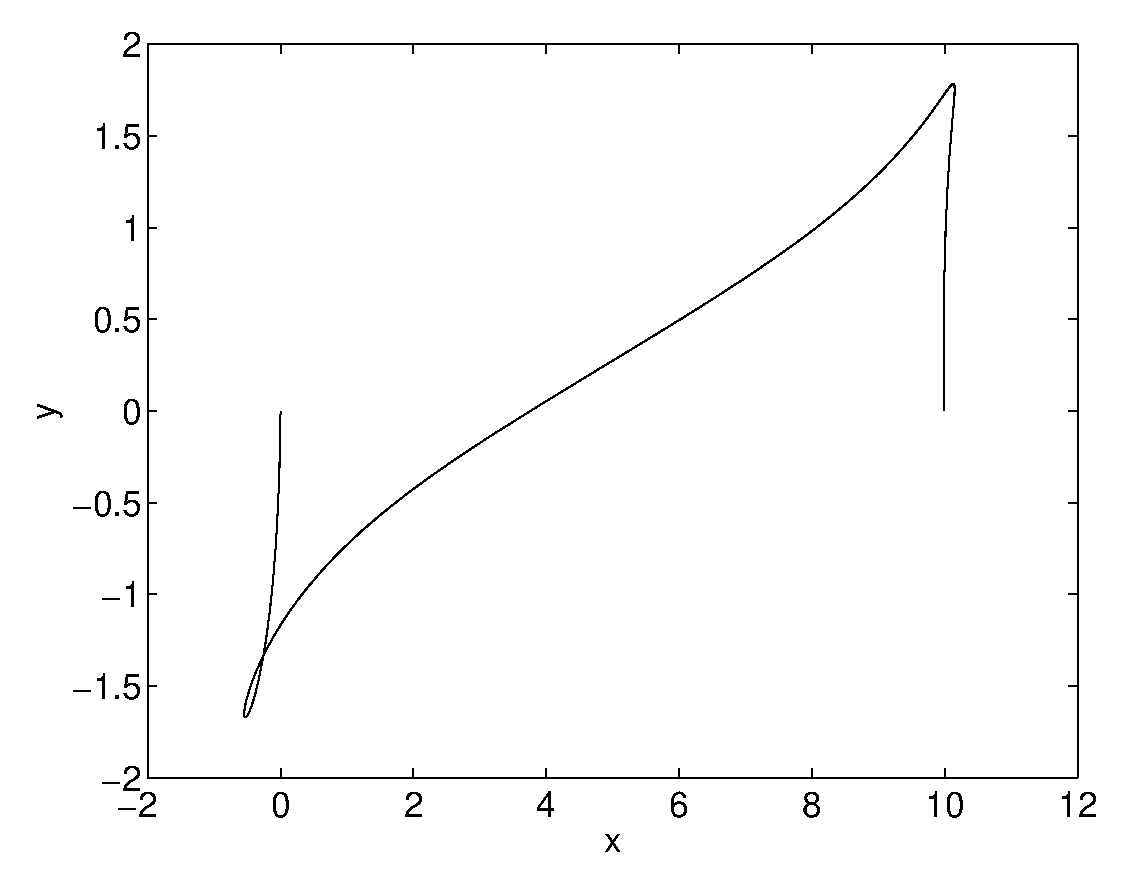
\includegraphics[height=0.3\textheight]{img/final_1_1_20_path.eps}
\caption{path}
\end{subfigure}

\begin{subfigure}[b]{\textwidth}
\centering
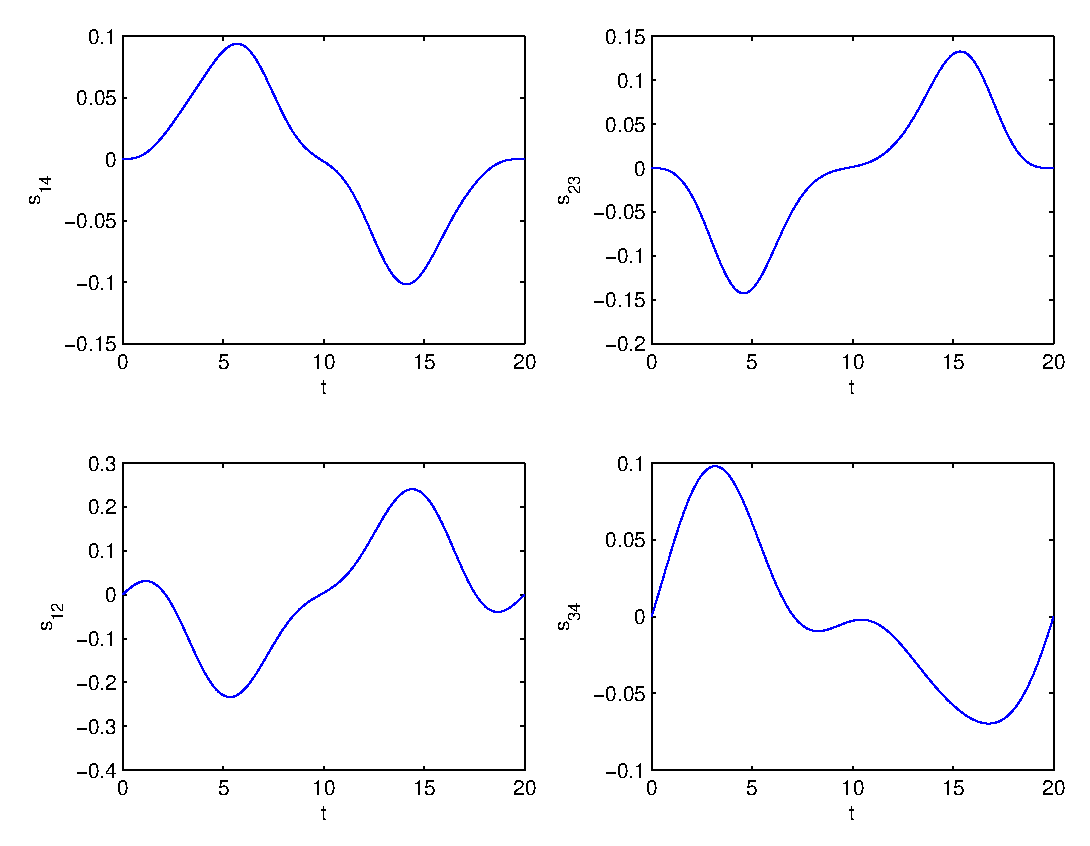
\includegraphics[height=0.3\textheight]{img/final_1_1_20_slips.eps}
\caption{slips}
\end{subfigure}

\begin{subfigure}[b]{\textwidth}
\centering
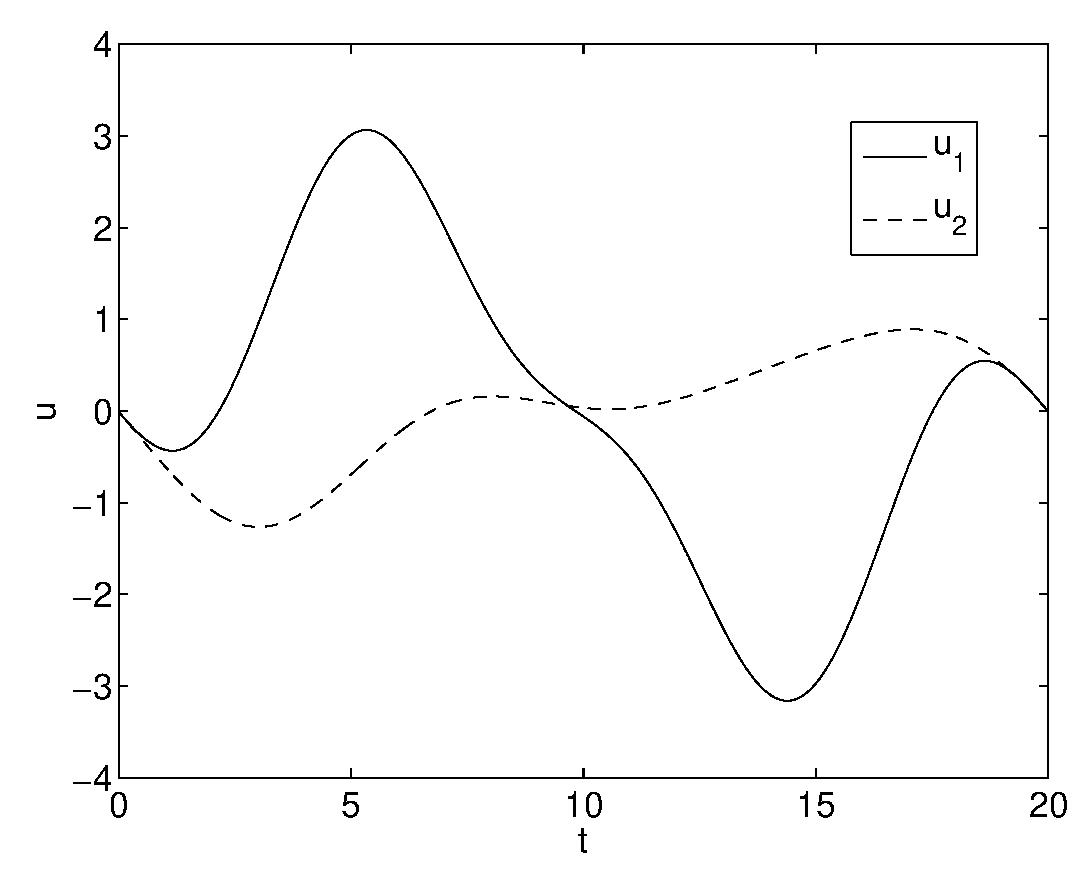
\includegraphics[height=0.3\textheight]{img/final_1_1_20_u.eps}
\caption{path}
\end{subfigure}
\caption{Mobile platform, $\epsilon=1$, $\tau=1$, $T=20$}
\label{fig:pl8}
\end{figure}

%%%%%%%%%%%%%%%%%%%%%%%%%%%%%%%%%%%%%%%%%%%%%%%%%%%%%%%%%%%%%%%%%%%%%%%%%%%%%%%%%%%%%%%%%%%
%%%%%%%%%%%%%%%%%%%%%%%%%%%%%%%%%%%%%%%%%%%%%%%%%%%%%%%%%%%%%%%%%%%%%%%%%%%%%%%%%%%%%%%%%%%
%%%%%%%%%%%%%%%%%%%%%%%%%%%%%%%%%%%%%%%%%%%%%%%%%%%%%%%%%%%%%%%%%%%%%%%%%%%%%%%%%%%%%%%%%%%
%%%%%%%%%%%%%%%%%%%%%%%%%%%%%%%%%%%%%%%%%%%%%%%%%%%%%%%%%%%%%%%%%%%%%%%%%%%%%%%%%%%%%%%%%%%
%%%%%%%%%%%%%%%%%%%%%%%%%%%%%%%%%%%%%%%%%%%%%%%%%%%%%%%%%%%%%%%%%%%%%%%%%%%%%%%%%%%%%%%%%%%

\subsection{Discontinuous friction model}
This model assumes that coefficients $\epsilon_i$ and $\tau_i$ in \eqref{eq:force_r} depend on the value of the slip. The point of such approach is to model the phenomenon of losing the traction. We will assume that for every friction force we have two values of the friction coefficient: high when the slip is less than the certain value (traction) and low otherwise (skid). This idea leads to the following formulae
\begin{equation*}
\begin{aligned}
\epsilon_i&=\begin{cases}
\epsilon_{high} &\mbox{if } |s| \leq d \\
\epsilon_{low} &\mbox{if } |s| > d
\end{cases}, &
\tau_i&=\begin{cases}
\tau_{high} &\mbox{if } |s| \leq d \\
\tau_{low} &\mbox{if } |s| > d
\end{cases},
\end{aligned}
\end{equation*}
where $i=1, 2, 3, 4$. The values used in simulations are: $\epsilon_{high}=10$, $\epsilon_{low}=5$, $\tau_{high}=3$, $\tau_{low}=1$. Unfortunately, there is no guarantee for the algorithm to converge for a discontinuous model and such situation takes place in this case. The plot of the error norm with respect to the iteration number is shown in the figure \ref{fig:error_discont}. It is clearly visible that the plot of the error norm is not monotonic. The reason why the endogenous configuration approach does not perform well here is the fundamental idea of the motion planning algorithm. It assumes that a small change in endogenous configuration results in a small change in the output function value. This statement is true for continuous models. On the contrary, when a model includes some discontinuities, even a small variation to the input may take the system to a distant point from the original one in the output space. Therefore, the error may increase in the next iteration of the algorithm. Note that decreasing the $\gamma$ parameter in equation \eqref{eq:endogen_num} will not solve this problem neither.
In other words, if the platform loses the traction in a different point than in the previous iteration it ends up in a place not related to the one supposed to be according to the algorithm, because actually the model has changed in the meanwhile.
\begin{figure}[htp]
\centering
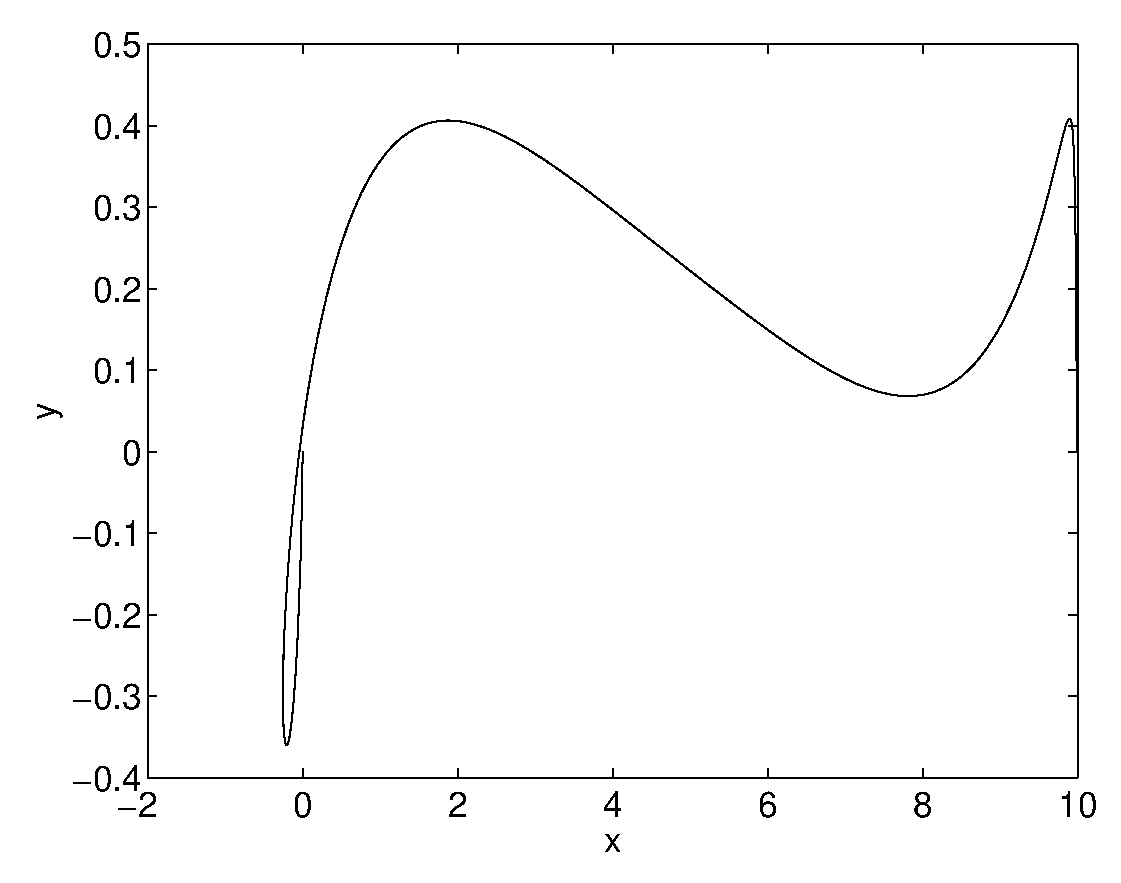
\includegraphics[height=0.3\textheight]{img/final_15_1_10_path.eps} %TODO make proper image
\caption{Error norm w.r.t iteration, discontinuous model of the platform}
\label{fig:error_discont}
\end{figure}

\section{Mobile manipulator}

When it comes to the manipulator,
its coordinates in task space $(\phi, \theta, \psi, y, z) $ should be equal to
$(-\frac{\pi}{2}, -\frac{\pi}{4}, \frac{\pi}{2}, 0, 0.2)$.
This corresponds to a parking manoeuvre with the manipulator
looking straight forward, observing the floor right in front of it.
